\documentclass{article}

\usepackage{fontspec}
\usepackage[hyphens]{url}
\usepackage[hidelinks]{hyperref}
\usepackage[normalem]{ulem}
\usepackage{siunitx}
\usepackage{graphicx}
\setmainfont{TeX Gyre Pagella}
\newcommand{\Vbat}{$V_{bat}$}
\newcommand{\Vout}{$V_{out}$}
\newcommand{\Vref}{$V_{ref}$}
\newcommand{\chippin}{\texttt}

% TODO: add SCP explanation
% TODO: understand and add 34V generator
\begin{document}
\section{About This Document}
This is my attempt to understand how the DC power board in the Game
Gear works. The information in this document is based on the MB3775
datasheet, the 2SB1301 datasheet, \textit{The Art of Electronics}, and
my own real-world tests in a separate circuit. I have not actually
opened my Game Gear to measure any voltages, so all this information
may be incorrect.

This document is also meant to be used alongside a schematic of the
power board. See Section \ref{sec:documents} for URLs for both
schematics and datasheets.

In this document, chip pins are \chippin{typeset like this} and
components, as well as voltages, are typeset like this: \Vref{}.

I claim no responsibility if you try to modify the board, tap a power
line, or something else completely, and your battery-guzzling handheld
releases the magic blue smoke. Be careful!

\section{Introduction}
The Game Gear has to supply 5 volts DC as well as reasonably
high-current 34 volts DC, all from a set of six AAs or a \qty{1}{A} DC
wall wart, \textit{and} has to be compact and not heat-producing. As a
result, the console doesn't use a '7805 regulator and a high-quality
DC inverter, but a low-power PWM chip and a few transistors.

I believe the power board is nearly identical or identical across all
console revisions.

\subsection{Where The Power Goes}
The \qty{5}{\volt} supply powers almost every component in the Game
Gear. This includes the Z80, both RAM chips, the cartridge ROM, the
VDP/PSG, the VDP to LCD picture circuitry, and even the florescent
tube (weird, but it's true). Most of these components are just silicon
in the two or one ASIC(s) on the main board, and the tube is driven
with an AC inverter and the large transformer, also on the main board.

The \qty{34}{\volt} supply is used, then, for just one thing: driving
the actual LCD. I'm not sure why the screen needs such high voltage,
especially at the low currents ($<$\qty{100}{\milli{}A}) that the
transistors on the power board can supply. This means, however, that
if you choose to install a new backlight, \textbf{do not cut the
  \qty{34}{\volt} line.} The screen still needs it, even if the
backlight doesn't.

\subsection{Test Circuit}
In figuring all this out, I used a small test circuit (Figure
\ref{fig:test_circuit_schematic}) built around the power outputs of an
Arduino Uno with a \qty{9}{\volt} supply. That supply is connected to
$Q_1$'s emitter through the Arduino's $V_{in}$ pin.

\begin{figure}
  \centering
  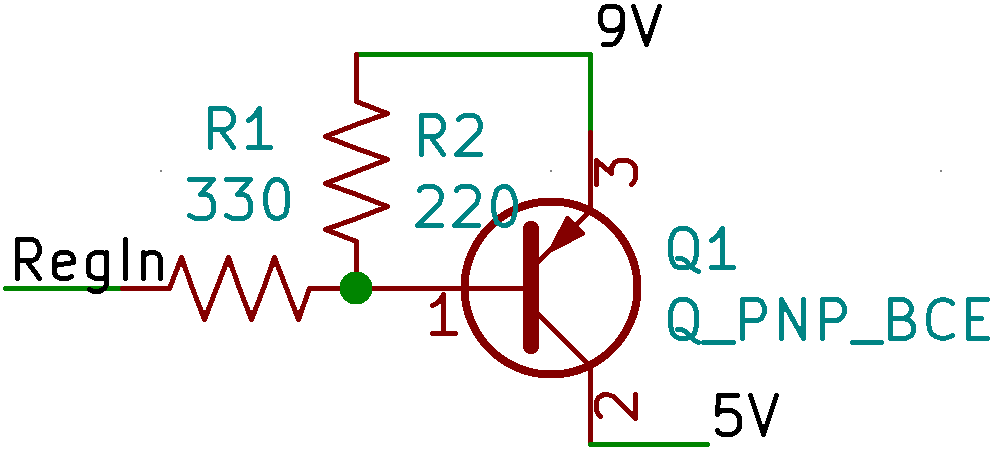
\includegraphics[width=\textwidth]{test_circuit_schematic}
  \caption{The schematic for my test circuit. Note that R1 is
    \qty{330}{\ohm} instead of \qty{360}{\ohm}, as I only had the
    former.}
  \label{fig:test_circuit_schematic}
\end{figure}


% TODO: take a picture of the test circuit.
\subsection{Signal and line names}
\begin{description}
\item[\Vbat{}] The positive voltage from the 6 batteries or the DC power
  jack. This is ideally \qty{9}{\volt}, but will vary. I think the
  power jack is ``prioritized,'' so to speak, over the batteries.
\item[\Vout{}] The final regulated \qty{5}{\volt} output, after the
  chip, transistor, coil ($L_2$), and decoupling capacitors.
\item[\Vref{}] The \qty{1}{\milli{}A} \qty{1.28}{\volt} supply from the
  MB3775. This is also present on the board connector, with the same
  name.
\end{description}

\section{Power Input}
Raw unregulated power can come from one of two sources on the Game
Gear: a), the 6 AAs, or b), the DC power jack. The AAs are connected
in series, for an optimal voltage of \qty{9}{\volt}.

The power jack, however, is a little more complicated. An American
Game Gear accepts a center-positive \qty{1.7}{\milli\meter} inner
diameter by \qty{4.75}{\milli\meter} outer diameter barrel plug, while
a European (and possibly Japanese?) Game Gear accepts a more common
\qty{2.1}{\milli\meter}/\qty{5.5}{\milli\meter}
\textbf{center-negative} plug. Note that the polarity is switched
between the two regions. I have no idea why Sega decided this was a
good idea.

On the power board, the positive line of the DC jack is connected
through diode $D_1$ to the positive line of the battery pack. The
negative line, naturally, goes to the main ground. I have no idea why
$D_6$ is on the schematic if it's labeled ``NOT USED''.

The positive and negative lines are then cleaned with the ferrite
beads $J_V$ and $J_G$. These are visible on the circuit board as the
long parallel vertical tubes to the lower right of the MB3775.

Finally, the switch will connect the power board's main supply to
either ground (to disable it completely) or to \Vbat{}. $C_{14}$ will
help settle any ripples created when the switch is turned on.

\subsection{Input Voltage}
I think this is something that is actually very confusing. The Game
Gear case labels the power jack as \texttt{DC 9V}. However, the Sega
power supply MK-2103, which is the official wall wart for the Game
Gear, is \qty{10}{\volt}. It's strange indeed, particularly if you
come from a world where precise voltage is important.

Fortunately, the exact voltage doesn't make all that much
difference, for a few reasons:

\begin{enumerate}
\item An alkaline AA will only be at \qty{1.5}{\volt} for the first
  few minutes of its life, at the discharge rate used by the Game
  Gear. From there, it will slowly drop to about \qty{1}{\volt}, where
  the voltage will drop sharply. This means that the voltage will be
  at about $\qty{1.3}{\volt} \times{} 6 = \qty{7.8}{\volt}$, give or
  take. This is clearly far beneath the optimal \qty{9}{\volt} that
  Sega suggests one should be using.

  Source: \url{https://www.powerstream.com/AA-tests.htm}, the
  \qty{500}{\milli{}A} graph.
\item The MB3775 can operate from \qty{3.6}{\volt} to
  \qty{18}{\volt}. The innate nature of the error amplifier means that
  the value of $V_{CC}$ doesn't matter, as the amp output will adjust
  to compensate.
\end{enumerate}

\subsection{Compatible Plugs}
I do not have a European Game Gear, but I would assume that a
commonplace 9V wall wart, like an Arduino power supply, would work
fine. Of course, make sure the polarity is correct if you do this.

For a US Game Gear, I've had success using the CUI Devices model
\texttt{PP-014}. DigiKey carries this as part number
\texttt{CP-014-ND}. This plug fits and works perfectly.

\section{MB3775 Configuration}
The Fujitsu MB3775 is the heart of the whole power board. This chip is
low-power (\qty{1.3}{\milli{}A}), with a large input voltage range
(\qty{3.6}{\volt} to \qty{18}{\volt}), and short-circuit
protection. It is a switching regulator controller, in essence, a PWM
generator. It is powered directly from \Vbat{}.

\subsection{Oscillator Timing}
The oscillator timing pins, $C_T$ and $R_T$, are connected to ground
through $C_7$, \qty{680}{\pico\farad} capacitor, and $R_9$, a
\qty{47}{\kilo\ohm} resistor, respectively.

I'm not fully sure how the value of the components on these pins
matter. They set the amplitude, frequency, and cycle of the
internally-generated triangular waveform, but there's no simple
equation for the values like there is for other parts of the chip.

\subsection{Short Circuit Protection}
I'm confident that the Game Gear's short circuit protection is
actually the heart of a common mistake or rumor: the ASIC(s) on the
main board \emph{do not} protect the console from shorts. Instead, the
protection is all within the power board, and basically entirely
enclosed in the MB3775. The short circuit protection (SCP) circuitry
works like this (don't confuse the SCP circuitry with the
\chippin{SCP} pin):

\begin{enumerate}
\item The outputs of the error amplifiers are connected to the
  non-inverting inputs of the SCP comparator, which checks that input
  against an internally-generated \qty{1.1}{\volt} supply connected to
  the inverting input.
\item When the load is stable and not changing, the error amplifier's
  output will not fluctuate (the current draw is steady, and the
  voltage has stabilized). Under this condition, the \chippin{SCP} pin
  is kept at approximately \qty{50}{\milli\volt}.
\item If the load changes drastically due to a short circuit (the
  current becomes very high and resistance goes low), causing a
  voltage below \qty{1.1}{\volt} to be supplied to the non-inverting
  input, the SCP comparator will output a ``low'' signal, switching an
  internal transistor off. This will discharge the \chippin{SCP} pin,
  and the SCP comparator will charge capacitor $C_1$ by this formula:

\begin{displaymath}
  V_{PE} = \qty{50}{\milli\volt} + t_{PE} \times
  \frac{10^{-6}}{C_{PE}}
\end{displaymath}

where

\begin{displaymath}
  V_{PE} = \qty{0.65}{\volt}, C_{PE} = \qty{0.68}{\micro\farad}
\end{displaymath}

($V_{PE}$ is set within the chip) and

\begin{displaymath}
  C_{PE} = \frac{t_{PE}}{\qty{0.6}{\micro\farad}}
  \rightarrow{} t_{PE} = \qty{0.408}{\second}.
\end{displaymath}

\item Once $C_1$ has charged to voltage $V_{PE}$, an internal latch is
  set, which enables the under-voltage lockout circuit, turns off the
  output drive transistors, and sets the dead time to \qty{100}{\%}---all of
  which, together, disable any current output from the \chippin{OUT1}
  and \chippin{OUT2} pins.
\item Once the under-voltage lockout is enabled, the protection enable
  is released, but the latch won't reset until power is turned off.
\end{enumerate}

Point 1 means that if \emph{either} of the chip's outputs trigger the
short condition, then the entire chip will power down and stay off
until power is lost and re-applied.

Note: the SCP comparator will only output the ``low'' signal if the
voltage drops beneath \qty{1.1}{\volt} for $t_{PE} = 0.408$
seconds. This seems like a long time, especially since the example
circuits in the datasheet have $t_{PE} = \qty{0.06}{\second}$. I
suspect it's configured this way so that the initial load generated by
starting the florescent tube doesn't trigger the SCP. I wonder, then,
if an aging tube, which takes longer to start, could trigger the
protection by drawing current for longer than a new tube would.

Finally, $C_1$ is a tantalum capacitor because it has to hold a large
amount of charge, but the DC board is too packed with other parts
(like the gigantic $C_{13}$) for another electrolytic to fit.

\section{\qty{5}{\volt} Generation}
\subsection{Voltage Setting}
The \qty{5}{\volt} supply is created with the first PWM generator on
the MB3775 and transistor $Q_3$. A simple explanation is that the
output pin, \chippin{OUT1}, drives the base of $Q_3$, which behaves as
a collector or voltage follower, supplying the current from the
battery or DC power jack (which is provided through the emitter) at
\qty{5}{\volt}.

A more detailed explanation is as follows: the positive input of the
error amplifier, \chippin{IN1+}, is connected to the output of a
voltage divider created by $R_{14}$ and $R_{15}$, creating a negative
feedback loop. The negative input, \chippin{IN1-}, of the amplifier is
connected to \Vref, as described on page 12 of the MB3775 datasheet,
creating a positive voltage on the output pin. The same page of the
datasheet contains this equation, relating the values of the resistors
in the divider to the output voltage:

\begin{displaymath}
  V_0 = V_{ref}(1+\frac{R_{15}}{R_{14}}) =
  1.28(1+\frac{\qty{20}{\kilo\ohm}}{\qty{6.8}{\kilo\ohm}})
  = 1.28(1+2.941) = \qty{5.045}{\volt}.
\end{displaymath}

However, be careful: the voltage on \chippin{OUT1} \textbf{is not
  \qty{5}{\volt}}. Based on my test circuit, I've found that if the
\chippin{OUT1} voltage is \qty{5}{\volt}, then the collector voltage
on $Q_3$ is close to \qty{9}{\volt}, far too high to drive
\qty{5}{\volt} components. Instead, the \chippin{OUT1} voltage is
likely under constant flux, remaining at about 2 to 3 volts, as
dictated by the collector voltage.

Note that $R_{14}$ and $R_{15}$ are \qty{1}{\%} accuracy resistors, to
ensure that the output voltage from the chip is stable at
\qty{5}{\volt} or very close.

My test circuit also shows that the collector voltage is dependent on
the base current. This makes sense, given $I_C = h_{FE}I_B$ and Ohm's
Law. Assuming the load stays the same, increasing the current will
also increase the voltage, and vice versa. This means that the chip is
likely controlling how much current is sunk into the \chippin{OUT1}
pin, based on the signal into \chippin{IN1+}.

\subsection{Diode $D_3$, Coils $L_2$ and $L_3$, Caps $C_{12}$ and
  $C_{13}$}
Although it might seem that $D_3$ is present to ``prevent
collector-base conduction on negative swings'' if the load swings
below ground, as described in Section 2.02 of \textit{The Art of
  Electronics}, I believe this is
wrong. \url{https://electronics.stackexchange.com/a/159151} says that
if the collector voltage flows higher than the base voltage (for a
PNP), then the base-collector junction will become forward biased,
allowing current present on the collector to flow into the base and
damage the chip, as well as possibly the batteries and anything on the
main board connected to \Vbat. However, this doesn't take into account
the fact that the diode is installed with the arrow pointing
\emph{toward} the collector, and since the other side goes to ground,
the only way for the diode to not be reverse biased is if the
collector voltage drops below ground (technically, 0.6 volts above
ground). I see no way this could happen, because the chip is
configured to only create positive voltage, and the voltage divider
between \Vbat{} and \chippin{OUT1} will always drive the voltage above
0.

As such, I believe this explanation is correct:

The diode likely exists to prevent possible damage caused by $L_2$ or
$L_3$ (the latter is on the \qty{34}{\volt} circuit). For example,
when the power is turned off, the coils will still hold charge and may
create negative voltage. This will disperse outward, and the diode
will allow the voltage to equalize by becoming forward biased, and
prevent damage to any part of the circuit.

The capacitors $C_{12}$ and the very large electrolytic $C_{13}$ are
simply power-supply filter capacitors, present to eliminate
ripples. These ripples could be caused by $L_2$, or by an unclean
AC power supply, like a cheap wall wart.


\subsection{Error Amp Frequency Characteristic}
Figure 22 on page 21 of the MB3775 datasheet shows the feedback pin,
FB1, going to ground through a capacitor $C_P$. In our case, $C_P$ is
a \qty{0.1}{\micro\farad} capacitor, likely of some special type,
given the ``K'' marking on the schematic. However, this is really just
a default value. The resistors in the MB3775 set the high-frequency
gain to \qty{0}{\decibel}, and a \qty{0.1}{\micro\farad} capacitor
sets the gain between \qty{20}{\kilo\hertz} and \qty{5}{\mega\hertz}
to \qty{0}{\decibel}. In other words, Sega has made the gain 0 for any
part of the PWM wave.

\subsection{Max Duty Cycle}
The max duty cycle is tuned with the \chippin{DTC1} pin. Page 14 of
the datasheet shows that this is accomplished with another voltage
divider, in our case, made with $R_{10}$ and $R_{11}$, which are $R_a$
and $R_b$ respectively. Given

\begin{displaymath}
  V_{dt} = \frac{R_b}{R_a+R_b} \times{} V_{ref} =
  \frac{\qty{12}{\kilo\ohm}}{\qty{33}{\kilo\ohm} + \qty{12}{\kilo\ohm}} \times{}
  \qty{1.28}{\volt} = \qty{0.341}{\volt},
\end{displaymath}

\noindent
we find

\begin{displaymath}
  \mathrm{Duty Max \%} = \frac{\qty{1}{V} - V_{dt}}{\qty{0.6}{V}}
  \times{} 100 = \qty{109}{\%}.
\end{displaymath}

I believe this is just setting the duty cycle of the PWM output to
\qty{100}{\%}, or always on. This way, the output of the regulator and $Q_3$
is a steady 5 volts. The fact that there's an extra \qty{9}{\%} of headroom
likely ensures that the duty cycle is always maximum even if resistor
values change, due to temperature changes or natural inaccuracies.

Note that the graph on datasheet page 15 shows that a $V_{dt}$ voltage
beneath \qty{0.4}{\volt} will create a duty cycle of \qty{100}{\%}.

\section{\qty{34}{\volt} Generation}
The \qty{34}{\volt} supply is DC. It is used to power the LCD, even
though it seems more logical to use it to power the tube. Instead, the
\qty{5}{\volt} supply is DC-inverted, converted to AC, and stepped up
with the large transformer, all on the main board.

\subsection{Voltage Setting}
$R_7$ and $R_8$ control the output voltage in a fashion identical to
that of the \qty{5}{\volt} circuit:

\begin{displaymath}
  V_0 = V_{ref}(1+\frac{R_7}{R_8}) =
  1.28(1+\frac{\qty{110}{\kilo\ohm}}{\qty{4.3}{\kilo\ohm}}) = \qty{34.024}{\volt}
\end{displaymath}

\subsection{Max Duty Cycle}
First, the max duty cycle is set to

\begin{displaymath}
  \frac{\qty{1}{\volt} - V_{dt}}{\qty{0.6}{\volt}} \times{} 100 = \qty{70.67}{\%}
\end{displaymath}

\noindent
where

\begin{displaymath}
  V_{dt} = \frac{R_b}{R_a+R_b} \times{} V_{ref} =
  \frac{\qty{27}{\kilo\ohm}}{\qty{33}{\kilo\ohm} +
    \qty{27}{\kilo\ohm}} \times \qty{1.28}{\volt} = \qty{0.576}{\volt}.
\end{displaymath}

With this value of $V_{dt}$, we find (equation from datasheet page 15)

\begin{displaymath}
  \frac{V_O - V_{bat}}{V_O} \times{} 100 = \frac{34 - 9}{34} \times{}
  100 = \qty{73.5}{\%}.
\end{displaymath}

Now, the max duty cycle configuration becomes important. The above
equation means that as \Vbat{} drops, the duty cycle will
increase. Without the max duty cycle configured, the duty cycle would
just increase without limit. With the maximum, it can never get higher
than \qty{73.5}{\%}.

\subsection{Error Amplifier Frequency Characteristic}
$C_3$ is identical to $C_8$, and so the gain between
\qty{20}{\kilo\hertz} and \qty{5}{\mega\hertz} is
\qty{0}{\decibel}. In other words, no adjustment.

\subsection{Supporting Circuitry: the Step-up Switching Regulator}
The entire \qty{34}{\volt} circuit is a simple step-up switching
regulator, and it is very similar to the second example circuit in the
MB3775 datasheet. The \qty{70}{\%} duty cycle oscillator output from
\chippin{OUT2} controls the base of transistor $Q_1$. This transistor
is relatively high-voltage, with a maximum $V_{CB}$ of
\qty{-60}{\volt} and a maximum $V_{CE}$ of \qty{-50}{\volt}. However,
it makes up for this with a maximum $I_C$ of only
\qty{-100}{\milli{}A}.

When \chippin{OUT2} allows $Q_1$ to sink current, current will also
flow from its emitter to its collector. That collector output flows
into $Q_2$'s base. $Q_2$ is identical to $Q_1$, except that it is an
NPN transistor, not a PNP. $Q_2$ is also the transistor that is
responsible for actually creating the high-voltage output (\textit{The
Art of Electronics} section 6.19):

\begin{enumerate}
\item When $Q_2$'s emitter is near ground (the transistor has been
  switched on), the current through $L_1$ increases. 
\item When $Q_2$ switches off, as controlled by the MB3775 and $Q_1$,
  the voltage after $L_1$ will increase significantly, due to the
  nature of an inductor.
\item This increase in voltage will cause $D_2$ to become
  forward-biased, dumping current at high voltage into the
  \chippin{34V} connector pin and into $C_4$ and $C_5$.
\end{enumerate}

% TODO: What is the role of C5?
The particular value of \qty{34}{\volt} is selected and controlled by
the MB3775, of course.

\section{Current Draw}
My particular unit, which is a stock US VA1 837-9024, except for a
recap, draws about \qty{330}{\milli{}A} total when powered by a
\qty{9}{\volt} wall supply. I think most of this current is actually
drawn by the tube, and that the other circuitry does not draw much
current.

$Q_3$ has a maximum collector current of \qty{-3}{A}. This means it
can supply up to \qty{3}{A} from the emitter. Even if all
\qty{330}{\milli{}A} were on just the \qty{5}{\volt} line ($Q_3$'s
collector), there would still be over \qty{2.5}{A} of leeway for other
things to draw current.

However, it's probably not a good idea to draw from the
\qty{34}{\volt}. Transistors $Q_1$ and $Q_2$ have a maximum collector
current of \qty{-100}{\milli{}A} and \qty{100}{\milli{}A},
respectively. This comparatively small limit means that there probably
isn't much space to draw new current (and converting \qty{34}{\volt}
to something useful is difficult and inefficient anyway).

Finally, there's significant risk in drawing too much current from the
batteries or the DC jack. The average alkaline AA is only designed for
about a maximum current draw of \qty{1}{A}
(\url{https://www.eevblog.com/forum/projects/maximum-aa-battery-current-draw/}. Even
with less current than this, the batteries will likely start heating
up, which is obviously dangerous. Furthermore, drawing more current
will reduce the battery life to something even more measly.

\section{Documents}
\label{sec:documents}
\subsection{Datasheets}
\begin{description}
\item[MB3775 ($IC_1$)]
  \url{https://console5.com/techwiki/images/2/24/MB3775.pdf}
\item[FBA04VA450AB-00 ($J_V,J_G$)]
  \url{https://www.mouser.com/datasheet/2/396/leaded_i04_e-2307117.pdf}
\item[2SA812 ($Q_1$)]
  \url{https://www.electrokit.com/uploads/productfile/41017/2SA812.pdf}
\item[2SA1623 ($Q_2$)]
  \url{https://www.mouser.com/datasheet/2/258/2SC1623(SOT-23)-276330.pdf}
\item[2SB1301 ($Q_3$)]
  \url{https://www.renesas.com/us/en/document/dst/2sb1301-data-sheet}
\item[U1BC44 ($D_1$)]
  \url{https://toshiba.semicon-storage.com/info/docget.jsp?did=3193&prodName=U1BC44}
  
\item[HRF22 ($D_2,D_3$)]
  \url{https://datasheet.datasheetarchive.com/originals/distributors/Datasheets-316/565268.pdf}
\end{description}

\subsection{Schematics}
\label{sec:documents_schematics}
Console5 is probably the best source for schematics. The schematics
below are the ones you want if you're just going to be following along
with this document:
\begin{description}
\item[European VA0]
  \url{https://console5.com/techwiki/images/2/22/Game_Gear_VA0_Schematic_-_Power.png}
\item[Any region VA1]
  \url{https://console5.com/techwiki/images/8/87/Game_Gear_VA1_Schematic_-_DC-DC_and_Sound.png}.
\end{description}

Other schematics, for the main board or other parts, are at
\url{https://console5.com/wiki/Game_Gear#Schematics}.

The VA1 documents are printed in a font that doesn't seem to scale
well. To save you the work, these are the ones I had the most trouble
reading:

\begin{description}
\item[$D_1$] A Toshiba U1BC44 diode.
\item[$C_{13}$] A \qty{820}{\micro\farad} \qty{5.3}{\volt}
  electrolytic capacitor.
  
\item[$J_V$ and $J_G$] A pair of FBA04VA450AB-00
  \qty{3.5}{\milli\meter} \qty{45}{\ohm} ferrite beads. The way the
  schematic is laid out, it suggests that $J_V$ is a different part,
  but the tiny \texttt{*2} indicates that $J_V$ and $J_G$ are the same.
\end{description}
\end{document}
